\section{Visualización}
La red que se ha elegido para realizar esta práctica es la de \textit{Political
blogs}~\cite{data} de la
\href{http://www-personal.umich.edu/~mejn/netdata/}{página web de
Mark Newman}. Como su propio nombre indica, se trata de una red de blogs sobre
política de los Estados Unidos de América, donde los nodos son los blogs y las
aristas, los enlaces de una web a otra, tratándose entonces de un grafo
dirigido.

En la figura~\ref{fig:network-parties} se puede ver la representación gráfica de
la red. Se han utilizado los colores clásicos para representar las ideologías
políticas en los EEUU: el azul para la izquierda o los liberales y el rojo para
la derecha o los conservadores. El tamaño de un nodo refleja el grado total del
mismo, de forma que los nodos más grandes representan blogs que realizan/reciben
más enlaces. En total, tenemos 1490 nodos y 19025 aristas. En esta figura, vemos
como la red se ve muy pequeña, esto se debe a que hay muchos nodos que no tienen
relación con ningún otro, de manera que están aislados. En la imagen, estos
nodos forman un círculo casi imperceptible alrededor de la componente principal.

\begin{figure}
    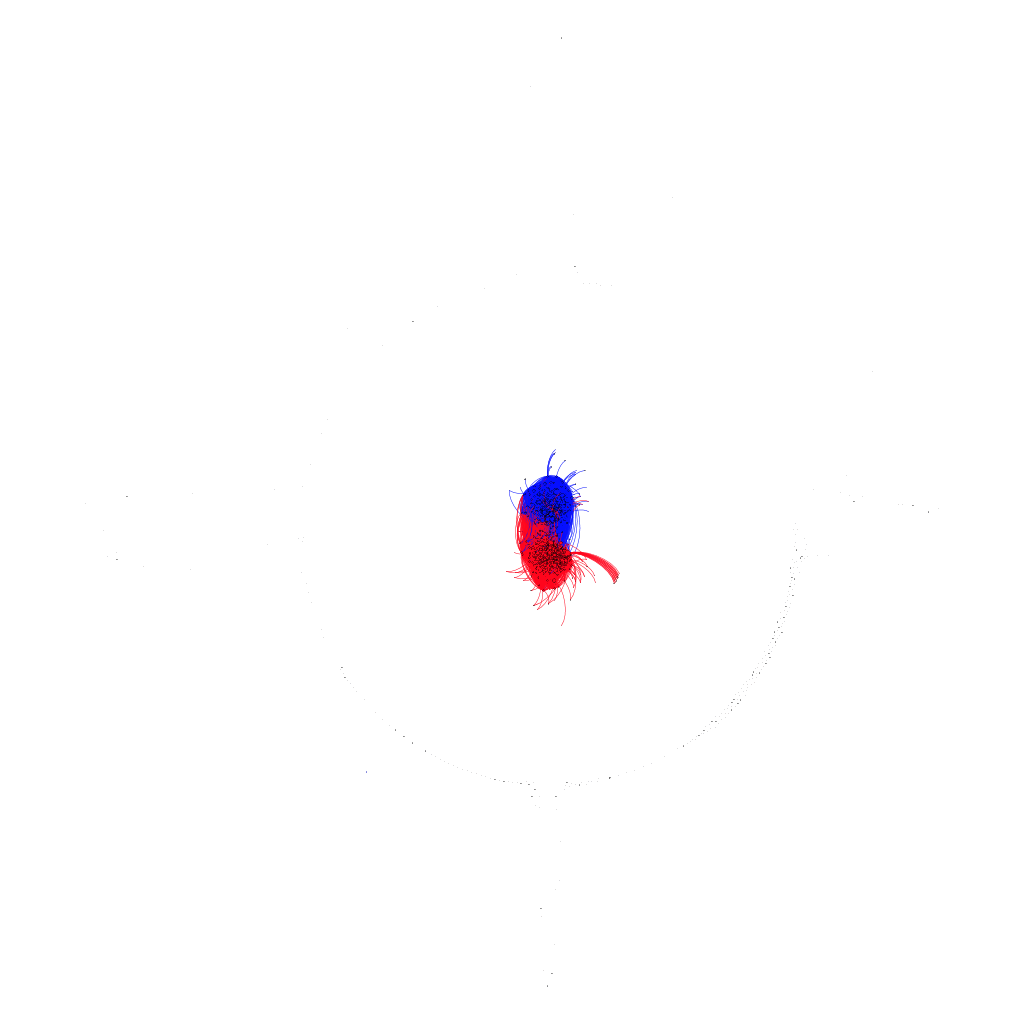
\includegraphics[width=\textwidth]{images/visualization/network/parties.png}
    \caption{Representación gráfica de la red}
    \label{fig:network-parties}
\end{figure}

Quedándonos solamente con esta componente gigante, obtenemos el grafo de la
figura~\ref{fig:network-giant-component}. Como era de esperar, los blogs de cada
ideología están fuertemente agrupados entre ellos, habiendo también bastantes
referencias de algunos blogs de cada ideología hacia la otra.

\begin{figure}
    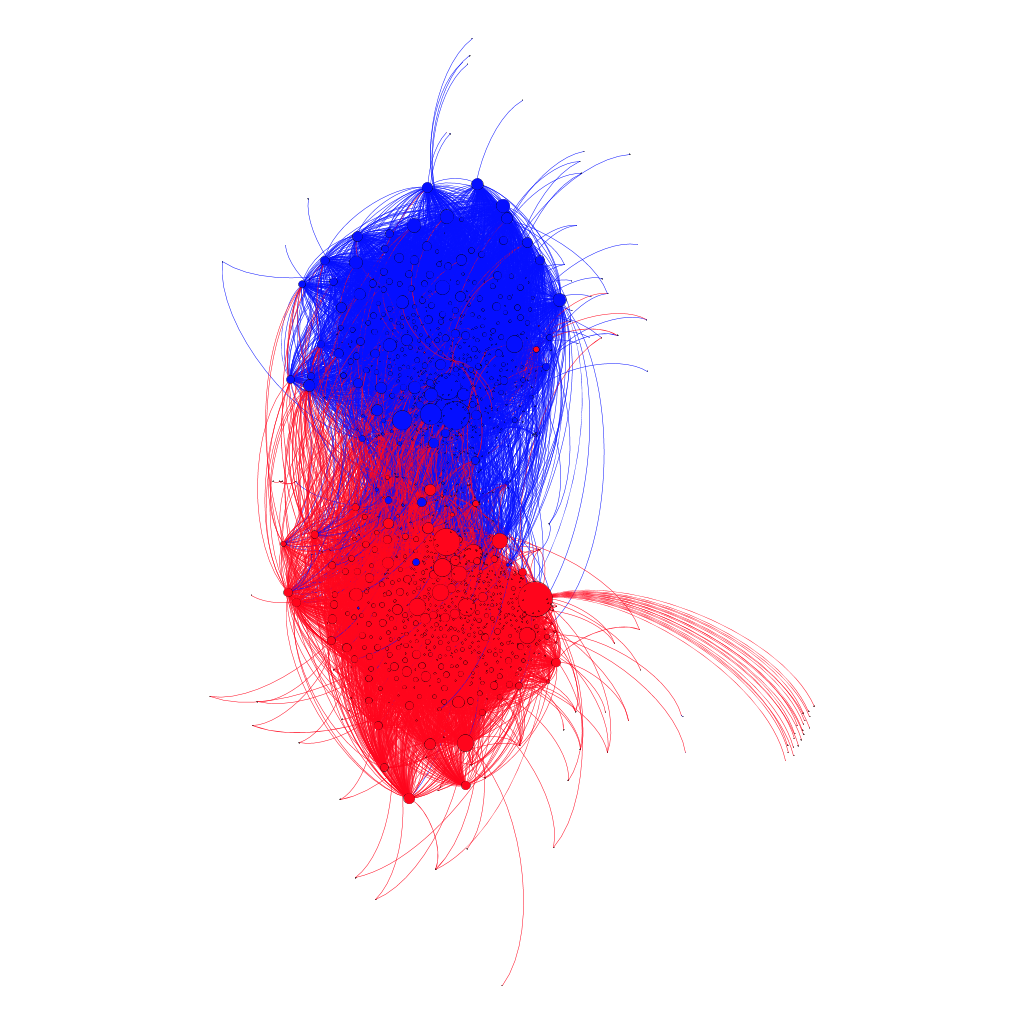
\includegraphics[width=\textwidth]{images/visualization/network/giant-component.png}
    \caption{Representación gráfica de la componente gigante}
    \label{fig:network-giant-component}
\end{figure}

\begin{table}[h!]
    \caption{Medidas obtenidas de la red}
    \label{tab:measurements}
    \begin{center}
    \begin{tabular}{ |c|c| }
        \hline
        Medida & Valor \\
        \hline
        Número de nodos $N$ & 1490 \\
        \hline
        Número de enlaces $L$ & 19025 \\
        \hline
        Número máximo de enlaces $L_{max}$ & 361931600 \\
        \hline
        Grado medio $\langle k \rangle$ & 12.768 \\
        \hline
        Densidad de grafo & 0.009 \\
        \hline
        Coeficiente medio de clustering $\langle C \rangle$ & 0.172 \\
        \hline
        Componentes conexas & 268 \\
        \hline
        Diámetro $d_{max}$ & 9 \\
        \hline
        Distancia media $d$ & 3.3902 \\
        \hline
    \end{tabular}
    \end{center}
\end{table}

Usando \textit{Gephi}, se han obtenido algunas medidas básicas de la red, las
cuales se pueden ver en la \ref{tab:measurements}. En las
figuras~\ref{fig:plot-degree-distribution} a
\ref{fig:plot-eccentricity-distribution} se muestran las distribuciones para
algunas medidas de la red como la centralidad y el grado de sus nodos.

\begin{figure}
    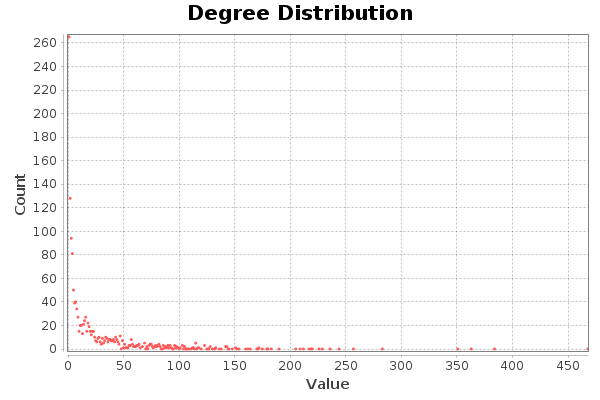
\includegraphics[width=\textwidth]{images/visualization/plots/degree-distribution.png}
    \caption{Distribución del grado total}
    \label{fig:plot-degree-distribution}
\end{figure}

\begin{figure}
    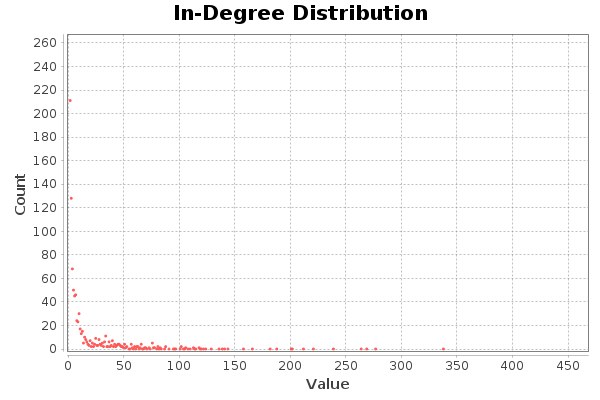
\includegraphics[width=\textwidth]{images/visualization/plots/indegree-distribution.png}
    \caption{Distribución del grado de entrada}
    \label{fig:plot-indegree-distribution}
\end{figure}

\begin{figure}
    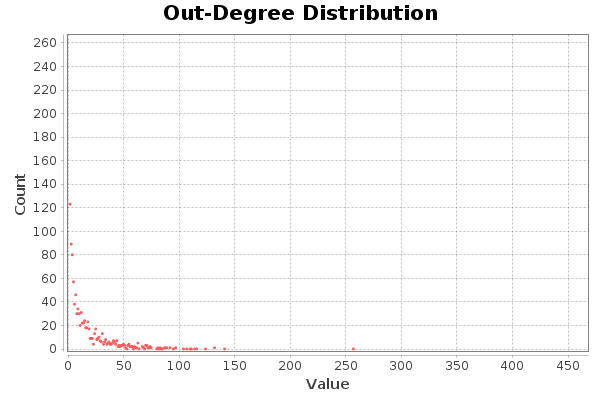
\includegraphics[width=\textwidth]{images/visualization/plots/outdegree-distribution.png}
    \caption{Distribución del grado de salida}
    \label{fig:plot-outdegree-distribution}
\end{figure}

\begin{figure}
    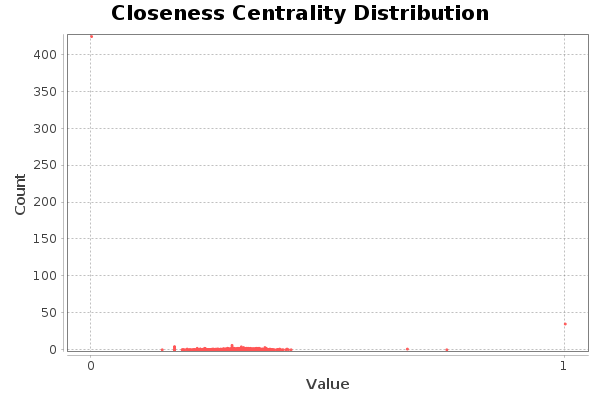
\includegraphics[width=\textwidth]{images/visualization/plots/closeness-centrality-distribution.png}
    \caption{Distribución de la centralidad de cercanía}
    \label{fig:plot-closeness-centrality-distribution}
\end{figure}

\begin{figure}
    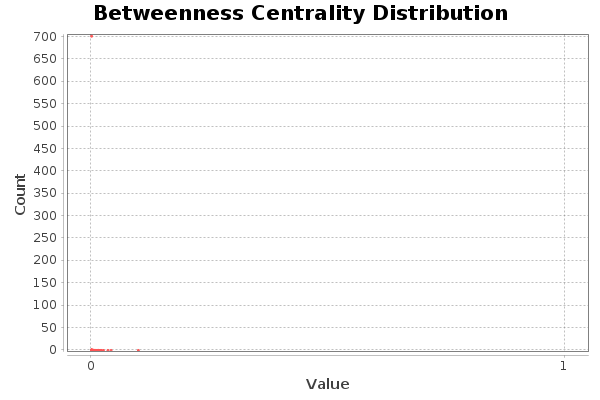
\includegraphics[width=\textwidth]{images/visualization/plots/betweenness-centrality-distribution.png}
    \caption{Distribución de la centralidad de intermediación}
    \label{fig:plot-betweenness-centrality-distribution}
\end{figure}

\begin{figure}
    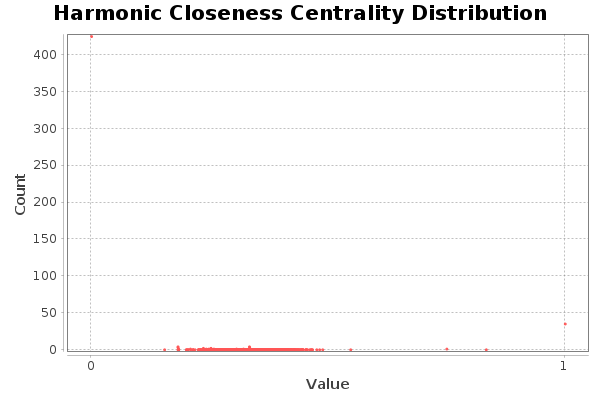
\includegraphics[width=\textwidth]{images/visualization/plots/harmonic-closeness-centrality-distribution.png}
    \caption{Distribución de la centralidad armónica de cercanía}
    \label{fig:plot-harmonic-closeness-centrality-distribution}
\end{figure}

\begin{figure}
    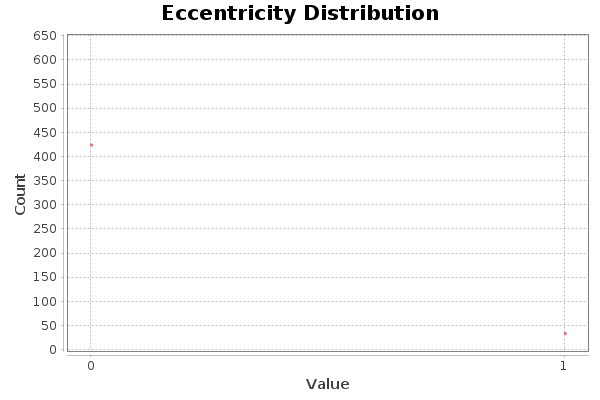
\includegraphics[width=\textwidth]{images/visualization/plots/eccentricity-distribution.png}
    \caption{Distribución de la excentricidad}
    \label{fig:plot-eccentricity-distribution}
\end{figure}
